\documentclass[11pt,a4paper]{article}

\usepackage[margin=2.2cm]{geometry}
\usepackage[T1]{fontenc}
\usepackage{lmodern}
\usepackage{amssymb}
\usepackage{xcolor}
\usepackage{tikz}
\usetikzlibrary{arrows.meta,positioning,fit,backgrounds}
\usepackage{booktabs}
\usepackage{tabularx}
\usepackage{enumitem}
\usepackage{listings}
\usepackage[most]{tcolorbox}
\usepackage{fancyhdr}
\usepackage[colorlinks=true,linkcolor=blue!50!black,urlcolor=blue!50!black]{hyperref}

\definecolor{local}{HTML}{2E7D32}
\definecolor{cloud}{HTML}{1565C0}
\definecolor{warn}{HTML}{C62828}
\definecolor{idea}{HTML}{6A1B9A}
\definecolor{soft}{HTML}{F5F5F5}

\newtcolorbox{concept}[1]{colback=idea!4,colframe=idea!70,fonttitle=\bfseries,title={Concept: #1},breakable}
\newtcolorbox{analogy}{colback=local!5,colframe=local!70,fonttitle=\bfseries,title={Analogy},breakable}
\newtcolorbox{why}{colback=cloud!4,colframe=cloud!70,fonttitle=\bfseries,title={Why it is done this way},breakable}
\newtcolorbox{caution}{colback=warn!4,colframe=warn!70,fonttitle=\bfseries,title={Watch out},breakable}
\newtcolorbox{exercise}{colback=soft,colframe=black!50,fonttitle=\bfseries,title={Check yourself},breakable}

\lstset{basicstyle=\ttfamily\small,backgroundcolor=\color{soft},frame=single,
        rulecolor=\color{black!25},columns=fullflexible,keepspaces=true,
        showstringspaces=false,breaklines=true}

\pagestyle{fancy}
\fancyhf{}
\lhead{\small Listen -- Learning Doc 04}
\rhead{\small Local Agent Internals}
\cfoot{\thepage}

\title{\textbf{Listen}\\[4pt]\large Learning Doc 04: Local Agent Internals\\
       \normalsize Audio, threads, events, feedback and timing}
\author{Detailed design, Section 3}
\date{13 October 2026}

\begin{document}
\maketitle

\begin{abstract}
\noindent Docs 01--03 decided \emph{what} the laptop agent does. This document designs
\emph{how it runs}: how sound gets from your microphone to a command, which parts work at the
same time (threads), how they talk (events and queues), how Listen answers you (chimes,
pop-ups, lowering other sounds), how it follows your microphone when you plug in a headset,
and how we will \emph{measure} that the whole trip takes under 1.5 seconds.
\end{abstract}

\tableofcontents
\newpage

% =====================================================================
\section{Decisions this section is built on}
\begin{center}
\renewcommand{\arraystretch}{1.2}
\begin{tabularx}{\textwidth}{l X}
\toprule
\textbf{Topic} & \textbf{Decision} \\
\midrule
Feedback      & Short sounds (chimes) plus a small pop-up at the bottom of the screen. No spoken voice. \\
Clearer audio & While Listen is capturing a command, other apps' sound is lowered, then restored. \\
Speed         & Under 1.5\,s from the end of your sentence to the action. Measure \texttt{tiny.en} and \texttt{base.en}, then choose. \\
Microphone    & Always the Windows \emph{default} input; follow it when it changes (headset plugged in). \\
\bottomrule
\end{tabularx}
\end{center}

% =====================================================================
\section{Doing several things at once: threads and queues}

The agent must listen to the microphone \emph{continuously}, while also transcribing, opening
apps, watching the foreground window and saving to the database. If these ran one after
another, the microphone would go deaf every time Listen opened Chrome.

\begin{concept}{Thread}
A \textbf{thread} is one line of work inside a program. A program with several threads can
wait for audio in one while it launches an app in another. (Doc~01 introduced the word; here
we use it for real.)
\end{concept}

\begin{concept}{Queue (message passing)}
Threads that share variables directly can corrupt each other's data (two threads updating the
same list at the same instant). The safe pattern is a \textbf{queue}: a thread-safe waiting
line. One thread \emph{puts} messages in; another \emph{takes} them out, one at a time, in
order. Threads never touch each other's data; they only pass messages. Python's built-in
\texttt{queue.Queue} does all the locking for us.
\end{concept}

\begin{analogy}
A restaurant kitchen: the waiter does not walk into the kitchen and stir the pot. They pin an
order ticket on the rail (the queue). The cook takes tickets in order. Waiter and cook never
get in each other's way, and nothing is lost when the kitchen is busy: tickets just wait.
\end{analogy}

\begin{concept}{The GIL (and why threads are still fine here)}
Python has a \textbf{Global Interpreter Lock}: only one thread runs \emph{Python} code at a time.
That sounds like it defeats threads, but our heavy work happens \emph{outside} Python:
speech recognition runs in compiled C++ (inside \texttt{faster-whisper}), and audio and
Windows calls are also native code. Those release the lock while they work. Most of our
threads spend their time \emph{waiting} (for audio, for a queue, for a timer), which costs
nothing.
\end{concept}

% =====================================================================
\section{The threads of the agent}

Each module owns one worker thread and one \textbf{inbox} queue. The event bus delivers events
into the inboxes of the modules that subscribed to that kind of event.

\begin{center}
\renewcommand{\arraystretch}{1.2}
\begin{tabularx}{\textwidth}{l X}
\toprule
\textbf{Thread} & \textbf{Job} \\
\midrule
Audio capture   & Receives 30\,ms chunks of sound from the microphone and pushes them into an audio queue. Does nothing else, so no sound is ever dropped. \\
Listener        & Runs voice detection and the wake word on those chunks; decides when a command starts and ends (Section~\ref{sec:states}); hands finished recordings on. \\
Transcriber     & Turns a recording into text with Whisper. Only one at a time. \\
Intent          & Matches text to a command (Doc~03). Fast, so it also handles confirmations. \\
Executor        & Runs actions and routines; owns the undo slot. \\
Feedback        & Plays chimes, shows pop-ups, lowers and restores other apps' volume. \\
Usage           & Checks the foreground window every 2\,s (Section~4 of the design). \\
Storage         & The only thread that writes to SQLite; saves events in small batches. \\
Housekeeping    & Every 2\,s: has the default microphone changed? Has a command file changed? \\
Hotkeys         & Push-to-talk key and the continuous-mode on/off key. \\
\bottomrule
\end{tabularx}
\end{center}

\begin{why}
\textbf{One writer for the database} avoids two threads writing at once (SQLite allows only one
writer at a time). \textbf{One transcriber} keeps CPU use predictable: if you speak twice
quickly, the second sentence simply waits its turn. And \textbf{audio capture does nothing but
capture}: anything slow there would cause gaps in the sound.
\end{why}

% =====================================================================
\section{Events: what travels on the bus}

Every event is a small, read-only record (a Python \texttt{dataclass}). Each carries the time it
was created, so we can measure every stage.

\begin{center}
\renewcommand{\arraystretch}{1.15}
\begin{tabularx}{\textwidth}{l l X}
\toprule
\textbf{Event} & \textbf{From} & \textbf{Means} \\
\midrule
\texttt{WakeWordDetected}      & listener   & ``Hey Jarvis'' heard \\
\texttt{CaptureStarted / Ended}& listener   & A command recording began / finished \\
\texttt{UtteranceCaptured}     & listener   & A finished recording, plus which mode produced it \\
\texttt{Transcribed}           & transcriber& The text, its confidence and how long it took \\
\texttt{HeardInContinuous}     & transcriber& Text heard in continuous mode (for the private log) \\
\texttt{IntentMatched}         & intent     & Command + filled slots + match confidence \\
\texttt{IntentNotMatched}      & intent     & Text + why (no pattern / below threshold) \\
\texttt{ConfirmationRequested} & intent     & ``Start DSA?'': waiting for yes/no \\
\texttt{CommandExecuted}       & executor   & Success, result, undo information, timings \\
\texttt{CommandFailed}         & executor   & What went wrong \\
\texttt{UndoPerformed}         & executor   & What was reversed (or ``can't undo'') \\
\texttt{ForegroundChanged}     & usage      & New app and cleaned title in front \\
\texttt{ModeChanged}           & hotkeys/intent & Wake word / continuous / off \\
\texttt{MicrophoneChanged}     & housekeeping & New default input device \\
\texttt{ModuleError}           & any        & A module hit an error (it keeps running) \\
\bottomrule
\end{tabularx}
\end{center}

% =====================================================================
\section{The listener as a state machine}\label{sec:states}

\begin{concept}{State machine}
A \textbf{state machine} is a thing that is always in exactly one \emph{state}, and moves
between states only on specific \emph{events}. Writing the listener this way makes every
situation explicit: ``what happens if you press push-to-talk \emph{while} it is waiting for a
yes/no?'' has one clear answer instead of a tangle of \texttt{if} statements.
\end{concept}

\begin{center}
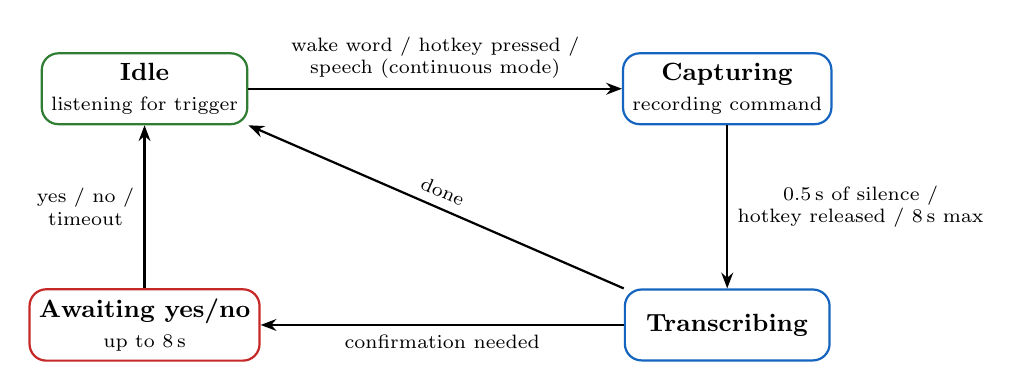
\begin{tikzpicture}[font=\small,
  st/.style={draw,rounded corners=6pt,minimum width=2.6cm,minimum height=0.9cm,align=center,fill=white,thick},
  arr/.style={-{Stealth[length=2mm]},thick},
  lab/.style={font=\scriptsize,align=center}]
\node[st,draw=local] (idle) at (0,0) {\textbf{Idle}\\\scriptsize listening for trigger};
\node[st,draw=cloud] (cap) at (7.4,0) {\textbf{Capturing}\\\scriptsize recording command};
\node[st,draw=cloud] (tr) at (7.4,-3) {\textbf{Transcribing}};
\node[st,draw=warn] (conf) at (0,-3) {\textbf{Awaiting yes/no}\\\scriptsize up to 8\,s};
\draw[arr] (idle) -- node[above,lab]{wake word / hotkey pressed /\\speech (continuous mode)} (cap);
\draw[arr] (cap) -- node[right,lab]{0.5\,s of silence /\\hotkey released / 8\,s max} (tr);
\draw[arr] (tr.north west) -- node[above,sloped,lab]{done} (idle.south east);
\draw[arr] (tr) -- node[below,lab]{confirmation needed} (conf);
\draw[arr] (conf) -- node[left,lab]{yes / no /\\timeout} (idle);
\end{tikzpicture}
\end{center}

\noindent The three listening modes differ only in \emph{what moves Idle to Capturing}:
\begin{itemize}[nosep]
  \item \textbf{Wake word}: the wake-word model fires (it only runs on chunks that voice
        detection marked as speech, which keeps it cheap).
  \item \textbf{Push-to-talk}: the hotkey is pressed; releasing it ends capture.
  \item \textbf{Continuous}: voice detection alone starts capture. The guardrails from Doc~03
        (standalone sentence, $\le$ 8 words, stricter thresholds) are applied after transcription.
\end{itemize}

\paragraph{The pre-roll buffer.} Voice detection needs a moment to be sure someone is speaking,
and you might start talking the instant you finish ``Hey Jarvis''. So the listener always
keeps the last \textbf{0.3\,s} of audio in a small rolling buffer and adds it to the front of
every recording. No first syllable is ever cut off.

\paragraph{Confirmations without a voice.} When a command needs confirmation, Listen plays a
distinct \emph{question} chime and shows a pop-up: ``Start DSA? Say yes or no''. For the next
8 seconds it listens \emph{without} needing the wake word. ``Yes'' runs it, ``no'' cancels it,
silence cancels it (with the ``cancelled'' chime).

% =====================================================================
\section{Feedback: chimes, pop-ups and lowering other sounds}

\subsection{Chimes}
Four short, clearly different sounds, played with Python's built-in \texttt{winsound} (no
extra download):
\begin{center}
\renewcommand{\arraystretch}{1.15}
\begin{tabular}{ll}
\toprule
\textbf{Chime} & \textbf{Meaning} \\
\midrule
listening   & wake word heard / recording started \\
done        & command executed \\
question    & waiting for yes / no \\
not caught  & didn't catch that / failed / can't undo / cancelled \\
\bottomrule
\end{tabular}
\end{center}
While a chime plays, the listener ignores the microphone for that fraction of a second, so
Listen never ``hears'' its own sound.

\subsection{Pop-ups}
A small Windows notification at the bottom right: ``Searching Google: what is an atom'',
``Didn't catch that'', ``Start DSA? Say yes or no''. These use the standard Windows
notification system, so they appear in the Action Center history too.

\subsection{Lowering other sounds (``ducking'')}
\begin{concept}{Audio ducking}
\textbf{Ducking} temporarily lowers other sounds so the important one is clear, like a
radio DJ's music dipping when they talk. Windows gives every app its own volume
\emph{session}, so Listen can lower Spotify and YouTube to 20\% without touching the master
volume, and put each one back exactly where it was.
\end{concept}

\begin{itemize}[nosep]
  \item \textbf{When:} from the moment capture starts (wake word heard / hotkey pressed) until
        transcription begins, typically 2--4 seconds.
  \item \textbf{Only other apps}: Listen's own chimes and the master volume are untouched, so
        ``volume up'' and its undo keep working normally.
  \item \textbf{Safe restore}: the original levels are written to a small file before
        ducking. If Listen crashes mid-duck, it restores them from that file on next start.
        Your music is never left stuck at 20\%.
\end{itemize}

\begin{caution}
\textbf{Ducking does not happen in continuous mode} (by design, open for discussion). In
continuous mode, capture starts whenever \emph{anyone} speaks, so ducking there would pump your
music down and up during every conversation in the room. Ducking stays for wake-word and
push-to-talk, where capture starts only when you asked for it.
\end{caution}

% =====================================================================
\section{Following your microphone}
Listen always records from the Windows \textbf{default input device}. Every 2 seconds the
housekeeping thread asks Windows which device that is. If it changed (you plugged in a
headset, or Windows switched to Bluetooth earbuds), Listen closes the old audio stream, opens
the new one, publishes \texttt{MicrophoneChanged}, and shows a pop-up: ``Now listening on:
Headset Microphone''. If no microphone exists at all, Listen waits and retries instead of
crashing.

\begin{caution}
Known Windows quirk to verify early: the audio library keeps a cached device list, so a
headset plugged in \emph{after} start-up may not appear until the library is restarted. The
housekeeping check therefore refreshes the library's device list before comparing. This is one
of the first things we test on your laptop, because it is easy to get wrong and annoying when
it is.
\end{caution}

% =====================================================================
\section{The 1.5-second budget}

\begin{concept}{Latency budget}
\textbf{Latency} is waiting time. A \textbf{budget} splits a total target into allowances per
stage, like splitting a monthly budget into rent and food. If the total is over, the budget
shows \emph{which} stage to fix.
\end{concept}

\begin{center}
\renewcommand{\arraystretch}{1.2}
\begin{tabularx}{\textwidth}{l r X}
\toprule
\textbf{Stage} & \textbf{Budget} & \textbf{Notes} \\
\midrule
Detect you stopped talking & 500\,ms & The silence the listener waits for. Often the \emph{biggest} item. \\
Speech-to-text             & 700\,ms & The number we must measure for \texttt{tiny.en} vs.\ \texttt{base.en}. \\
Matching                   & $<$5\,ms & Pure function (Doc~03). \\
Action starts              & 200\,ms & Launching the browser or app; the app's own loading time is not counted. \\
Feedback                   & 50\,ms  & Chime + pop-up. \\
\midrule
\textbf{Total}             & \textbf{$\approx$1.45\,s} & \\
\bottomrule
\end{tabularx}
\end{center}

\begin{why}
Notice that the first row is not the AI model at all: it is \emph{waiting for silence}. Make
it too short (200\,ms) and Listen cuts you off when you pause mid-sentence (``search\ldots what
is an atom''); too long and every command feels sluggish. Push-to-talk skips this wait
entirely, because releasing the key \emph{is} the end. Without a budget you would probably try
to speed up the model, the wrong place to start.
\end{why}

\subsection{How we will measure}
\begin{enumerate}[nosep]
  \item Record about 20 of your real commands once, as audio files.
  \item Run each file through \texttt{tiny.en} and \texttt{base.en} (both in the fast
        \texttt{int8} format): time per file, and words wrong per file.
  \item Pick the smallest model that is both under budget and accurate enough. Expectation
        (to be verified, not assumed): \texttt{base.en} is noticeably more accurate and still
        fits.
\end{enumerate}
\noindent The agent also stamps every event with a time, so the terminal shows the real
breakdown of every command you give, for example
\texttt{silence 500 | stt 420 | match 1 | action 160 | total 1081 ms}.

% =====================================================================
\section{Start-up, shut-down and failures}

\paragraph{Start-up order.} Load settings $\to$ load and validate command files $\to$ build
the app index $\to$ restore any volumes left ducked by a crash $\to$ load the speech and
wake-word models $\to$ open the microphone $\to$ start all threads $\to$ ``listening'' chime
and pop-up ``Listen is ready''. Each step prints a line in the terminal, so a failure points
at exactly one step.

\paragraph{Shut-down} (Ctrl+C or ``quit listening''). Stop accepting audio $\to$ let the
current command finish $\to$ restore ducked volumes $\to$ flush unsaved events to SQLite
$\to$ close.

\paragraph{When something breaks.} Every worker thread runs its loop inside an error handler.
An error in one module is logged, published as \texttt{ModuleError}, shown in the terminal, and
that module carries on with the next message. A \textbf{supervisor} checks every few seconds that
each thread is alive and restarts any that died. One bad command must never take the whole
assistant down.

\begin{concept}{Graceful degradation}
When part of a system fails, the rest keeps working with reduced ability instead of crashing.
No internet: commands still work, the command builder falls back to the form. No microphone:
Listen waits. Unknown app: ``CLion not found'', the rest of the routine still runs.
\end{concept}

% =====================================================================
\section{What you see in the terminal (v1 shell)}
\begin{lstlisting}
[09:41:02] ready  | mic: Realtek Microphone Array | mode: wake word | model: base.en
[09:41:15] wake word
[09:41:17] heard  "search what is an atom"   (confidence 0.93)
[09:41:17] match  search  query="what is an atom"  target=google  (1.00)
[09:41:17] done   open_url google.com/search?q=what+is+an+atom
           timing silence 500 | stt 412 | match 1 | action 140 | total 1053 ms
\end{lstlisting}
\noindent Every line is one event on the bus. When something misbehaves, you will see
\emph{which stage} did it, which is the whole point of building the terminal shell first.

% =====================================================================
\section{Glossary}
\begin{description}[style=nextline,leftmargin=1.2cm,itemsep=2pt]
  \item[Audio ducking] Temporarily lowering other sounds so one sound is clear.
  \item[Dataclass] A Python class that just holds named fields; used for events.
  \item[GIL] Python's lock letting one thread run Python code at a time; native code releases it.
  \item[Graceful degradation] Failing partially instead of completely.
  \item[Inbox] The queue in which a module receives its events.
  \item[Latency budget] A total time target split into per-stage allowances.
  \item[Pre-roll buffer] The last fraction of a second of audio, kept so recordings never start late.
  \item[Queue] A thread-safe waiting line for passing messages between threads.
  \item[State machine] Something that is always in one state and changes state only on events.
  \item[Supervisor] A watcher that restarts parts of a program that died.
  \item[Thread] One line of work inside a program.
\end{description}

% =====================================================================
\section{Check your understanding}
\begin{exercise}
\begin{enumerate}
  \item Why does the audio-capture thread do nothing except capture?
  \item Two threads both want to save an event at the same moment. How does the design prevent
        a conflict?
  \item In the state machine, what moves Listen from \emph{Idle} to \emph{Capturing} in each of
        the three modes?
  \item Why is ducking switched off in continuous mode?
  \item Listen crashes while Spotify is ducked to 20\%. What happens on the next start, and why
        is the original level safe?
  \item Your total latency is 2.1\,s and the breakdown says
        \texttt{silence 500 | stt 1350}. What do you try first?
  \item Why does push-to-talk feel faster than the wake word, even with the same model?
\end{enumerate}
\end{exercise}

\end{document}
